\section{Heuristic derivation of Advection Differential Equation}

\begin{frame}
	\begin{definition}[Average concentration]
		Let $h>0$, $h\ll 1$.
		We define the \emph{average concentration}
		\begin{math}
			\averageconcentration
		\end{math}
		in a space-time cell
		\begin{math}
			\left[
				x-\frac{1}{2}h,
				+x\frac{1}{2}h
				\right]
			\times
			\left[
				0,T
				\right]
		\end{math}.

		\begin{equation*}
			\averageconcentration=
			\dfrac{1}{h}
			\int_{x-\frac{1}{2}h}^{x+\frac{1}{2}h}
			u
			\left(
			s,t
			\right)
			\dl s.
		\end{equation*}
	\end{definition}

	\begin{definition}[Mass flux]
		The mass flux is the product of
		\begin{equation*}
			J_{x}=
			c
			v_{x}.
		\end{equation*}

		\begin{itemize}
			\item

			      $J_{x}$ is the mass flux in $x$-direction.

			\item

			      $c$ is the concentration of the substance.

			\item

			      $v_{x}$ is the velocity of the substance in the
			      $x$-direction.
		\end{itemize}
	\end{definition}

	\begin{theorem}[Conservation law]
		If the species is carried along by a flowing medium with
		velocity
		\begin{math}
			a\left(x,t\right)
		\end{math},
		then the mass conservation law
		implies that the change of
		\begin{math}
			\averageconcentration
		\end{math}
		per
		unit of time is the net balance of inflow and outflow over
		the cell boundaries,
		\begin{equation*}
			\diffp{\averageconcentration}{t}=
			\dfrac{1}{h}
			\left[
				a
				\left(
				x-\frac{1}{2}h,t
				\right)
				u
				\left(
				x-\frac{1}{2}h,t
				\right)-
				a
				\left(
				x+\frac{1}{2}h,t
				\right)
				u
				\left(
				x+\frac{1}{2}h,t
				\right)
				\right].
		\end{equation*}
	\end{theorem}
\end{frame}

\begin{frame}
	\frametitle{Numerical Quadrature~(\citeauthor[p.~9]{Hundsdorfer2003})}

	\begin{definition}[Advection equation]
		\begin{equation*}
			\diffp{\concentration}{t}+
			\diffp{a\left(x,t\right)\concentration}{x}=
			0.
			% u_{t}+du_{x}=0.
		\end{equation*}
	\end{definition}

	\begin{definition}[Diffusion equation]
		\begin{equation*}
			\diffp{\concentration}{t}=
			\diffp{}{x}
			\left(
			d\left(x,t\right)\diffp{\concentration}{x}
			\right).
			% u_{t}=du_{xx}.
		\end{equation*}
	\end{definition}

	\begin{figure}[ht!]
		\centering
		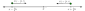
\includegraphics[width=.6\paperwidth]{deduction}
	\end{figure}
\end{frame}

\begin{frame}
	\begin{theorem}[Mass conservation law]
		If $\concentration$ is a concentration and
		\begin{equation*}
			M\left(t\right)\coloneqq
			\int_{0}^{1}
			u\left(x,t\right)
			\dl x
		\end{equation*}
		represents the mass in $\left[0,1\right]$ at time $t$, then
		$M$ is a conserved quantity.
	\end{theorem}

	\begin{proof}
		\begin{align*}
			\diff{M\left(t\right)}{t} & =
			\int_{0}^{1}
			u_{t}\left(x,t\right)
			\dl x=
			\int_{0}^{1}
			\left(
			-au_{x}\left(x,t\right)+
			du_{xx}\left(x,t\right)
			\right)\dl x                  \\
			                          & =
			-a\left(
			u\left(1,t\right)-
			u\left(0,t\right)
			\right)+
			d\left(
			u_{x}\left(1,t\right)-
			u_{x}\left(0,t\right)
			\right)=0.
		\end{align*}
	\end{proof}
\end{frame}

\section{The Advection Problem in One Dimension}

\begin{frame}
	\begin{definition}[space-time grid]
		Let $d\in\mathbb{N}$, $\Omega=\left(0,1\right)^{d}$, and $T>0$.
		For $K, N\in\mathbb{N}$, we set $\tau=\frac{T}{K}$ and
		$h=\frac{1}{N+1}$.
		We define the \emph{space-time grid domain}
		\begin{equation*}
			\overline{\mathcal{C}}^{\tau}_{h}=
			\overline{\Omega}_{h}\times
			{\left[0,T\right]}_{\tau}=
			\left\{
			\left(\mathbf{x},t_{k}\right)\mid
			\mathbf{x}\in\overline{\Omega}_{h},
			t_{k}=k\tau,
			k\in\left\{0,\dotsc,K\right\}
			\right\},
		\end{equation*}
		where we recall that
		\begin{math}
			\overline{\Omega}_{h}=
			\overline{\Omega}\cap
			\mathbb{Z}^{d}_{h}
		\end{math}.
		We define the \emph{discrete interior} of $\overline{C}^{\tau}_{h}$ to be
		\begin{equation*}
			\mathcal{C}^{\tau}_{h}=\Omega_{h}\times
			\left(0,T\right)_{\tau}.
		\end{equation*}
	\end{definition}

	\begin{definition}[space-time grid functions]
		Let $\mathcal{C}^{\tau}_{h}$ be a space-time grid domain.
		We denote by
		\begin{equation*}
			\mathcal{V}
			\left(
			\overline{\mathcal{C}}^{\tau}_{h}
			\right)=
			\left\{
			v\mid
			\overline{C}^{\tau}_{h}\to\mathbb{R}
			\right\}
		\end{equation*}
		be the space of \emph{space-time grid functions}.
		The spaces
		\begin{equation*}
			\mathcal{V}
			\left(
			\mathcal{C}^{\tau}_{h}
			\right),
			\mathcal{V}
			\left(
			\partial_{L}\mathcal{C}^{\tau}_{h}
			\right)
		\end{equation*}
	\end{definition}
\end{frame}

\begin{frame}
	\begin{definition}[space-time discrete norms]
		Let $d\in\left\{1,2\right\}$, $p\in\left[1,\infty\right]$, and
		$q\in\left[1,\infty\right)$.
		We define the \emph{space-time} norm
		\begin{equation*}
			\left\|
			v
			\right\|_{L^{q}_{\tau}\left(L^{p}_{h}\right)}=
				{\left(\tau
					\sum_{k=1}^{K}
					\left\|v^{k}\right\|^{q}_{L^{p}_{h}}
					\right)}^{\frac{1}{q}}
		\end{equation*}
		and
		\begin{equation*}
			\left\|
			v
			\right\|_{L^{\infty}_{\tau}\left(L^{p}_{h}\right)}=
			\max^{K}_{k=0}
			{\left\|
			v^{k}
			\right\|}_{L^{p}_{h}}
		\end{equation*}
	\end{definition}
\end{frame}

\begin{frame}
	\begin{definition}[Péclet number]
		Consider the simple constant-coefficient advection-diffusion
		equation
		\begin{equation*}
			u_{t}+
			au_{x}=
			du_{xx},\quad
			t>0,\quad
			0<x<L,
		\end{equation*}
		with the given initial profile $u\left(x,0\right)$.
		If $d>0$ we need boundary conditions at $x=0$ and $x=L$,
		such as Dirichlet conditions.
		On the other hand, for the pure advection problem we need
		only to prescribe the solution at the \emph{inflow} boundary,
		that is, at $x=0$ if $a>0$ and $x=L$ if $a<0$.
		If $d>0$ but $d\approx0$, or more precisely if the
		\emph{Péclet number}
		\begin{equation*}
			\left|a\right|\frac{L}{d}
		\end{equation*}
		is large, the Dirichlet condition at the outflow boundary
		will give rise to a \emph{boundary layer}.

		If the Péclet number $\left|a\frac{L}{d}\right|$ is large,
		the problem is called \emph{singularity perturbed}.
		% It is assumed that $d>0$, excluding the pure advection case.
		% where $L$ is the length of the spatial interval.
	\end{definition}
\end{frame}
